\documentclass[conference]{IEEEtran}
\usepackage{cite}
\usepackage{amsmath,amssymb,amsfonts}
\usepackage{algorithmic}
\usepackage{graphicx}
\usepackage{textcomp}
\usepackage{xcolor}
\usepackage{float}
\usepackage{tikz, pgfplots}
\def\BibTeX{{\rm B\kern-.05em{\sc i\kern-.025em b}\kern-.08em
    T\kern-.1667em\lower.7ex\hbox{E}\kern-.125emX}}

\pgfplotsset{compat=newest}

\begin{document}

\title{Conference Paper Title\\

\author{\IEEEauthorblockN{Tevin Hendess}
\IEEEauthorblockA{\textit{Computer Engineering Department} \\
\textit{Rochester Institute of Technology}\\
Rochester, NY USA \\
twh4619@rit.edu}
\and
\IEEEauthorblockN{Adam Schultzer}
\IEEEauthorblockA{\textit{Computer Engineering Department} \\
\textit{Rochester Institute of Technology}\\
Rochester, NY USA \\
ajs1539@rit.edu}
}
}

\maketitle

\begin{abstract}
The purpose of this exercise was to practice using an opto-isolator to detect changes in the reflection of light within a tube. 
This was accomplished by connecting the OPB745 photo-transducer to the necessary resistors and placing it in the tube and measuring
the voltage and current to see how the values changed as the distance from the sensor to the reflective surface varied. Further tests
were conducted with an inverter introduced into the circuit while the resulting waveform was recorded on an oscilloscope.
\end{abstract}

\section{Design Methodology}

Before constructing the circuit which would be used to test the opto-isolator and measure its output, the correct resistor values
had to be determined from the OPB745 datasheet along with the anticipated voltage values. In doing this, an expected "shape" for the
voltage and current graphs could be determined which allowed for verification as testing was conducted. The resistor value was
calculated according to the equation shown below.

\begin{equation}
    R_F=\frac{5V-V_{LED}}{I_{F_{MAX}}}=\frac{5-1.7}{0.04}=\frac{3.3}{0.04}=82.5\Omega
\end{equation}

As shown in Equation 1, the required resistor value for the LED is 82.5$\Omega$. This value is based on the total voltage through the
circuit (5V) and the voltage drop across the LED (1.7V as specified by the datasheet).

Another important part of the design was determining the expected values and pattern of an output from the photo-transducer. This was
done by examining the OPB745 datasheet which contained a graph of the output current at different distances from the reflective source.
A table of these values is shown in Table \ref{ExampleTable}

\begin{table}[H]
    \centering
    \caption{Add Your Caption Above the Table}
    \label{ExampleTable}
    \begin{tabular}{|c|c|cc|}
    \hline
                           &                        & \multicolumn{2}{c|}{\textbf{$R_{L1}$ = 10k}}                                                                   \\ \hline
    \textbf{Distance (in)} & \textbf{Distance (mm)} & \multicolumn{1}{c|}{\textbf{$V_{Out}$ (V)}} & \textbf{\begin{tabular}[c]{@{}c@{}}$I_{RL}$\\ (mA)\end{tabular}} \\ \hline
    0.0                    & 0.0                    & \multicolumn{1}{c|}{2.5}                    & 0.50                                                             \\ \hline
    0.05                   & 12.7                   & \multicolumn{1}{c|}{6.25}                   & 1.25                                                             \\ \hline
    \end{tabular}
\end{table}

\section{Results and Analysis}

As a result of testing the circuit with various reflection distances, it was able to be
determined what an ideal testing distance would be, using both a 10k$\Omega$ and 20k$\Omega$ resistance. 
The results of these tests are shown in Table \ref{distanceVoltageCurrent}.

\begin{table}[H]
    \centering
    \caption{Phototransistor Voltage and Current at Various Distances}
    \label{distanceVoltageCurrent}
    \begin{tabular}{|c||c|c||c|c|}
        \hline
         & \multicolumn{2}{c||}{$R_{L1}$ = \textbf{10k}} & \multicolumn{2}{c|}{$R_{L1}$ = \textbf{20k}} \\
        \hline
        Distance & $V_{out}$ (V) & $IRL$ (mA) & $V_{out}$ (V) & $IRL$ (mA) \\
        \hline
        0 & 4.919 &   0.008077383 & 4.81 &   0.009462151 \\
        1 & 3.175 &   0.181990427 & 1.225 &  0.187998008 \\
        2 & 0.727 &   0.426106901 & 0.7372 & 0.212290837 \\
        3 & 0.71 &    0.427802154 & 0.6984 & 0.214223108 \\
        4 & 0.729 &   0.425907459 & 0.6831 & 0.21498506 \\
        5 & 0.771 &   0.421719186 & 0.6874 & 0.214770916 \\
        6 & 0.817 &   0.41713203 & 0.6971 &  0.214287849 \\
        7 & 1.652 &   0.333865178 & 0.7156 & 0.213366534 \\
        8 & 2.563 &   0.243019545 & 0.735 &  0.212400398 \\
        9 & 3.126 &   0.186876745 & 0.7514 & 0.211583665 \\
        10 & 3.42 &   0.157558835 & 0.765 &  0.210906375 \\
        11 & 3.871 &  0.112584763 & 0.7899 & 0.209666335 \\
        12 & 4.038 &  0.095931392 & 0.8059 & 0.208869522 \\
        13 & 4.2167 & 0.078111288 & 0.82 &   0.208167331 \\
        14 & 4.274 &  0.072397288 & 0.8802 & 0.205169323 \\
        15 & 4.319 &  0.067909852 & 1.346 &  0.181972112 \\
        20 & 4.576 &  0.042281611 & 3.43 &   0.078187251 \\
        25 & 4.656 &  0.034303949 & 4.078 &  0.045916335 \\
        30 & 4.641 &  0.035799761 & 4.243 &  0.037699203 \\
        35 & 4.58 &   0.041882728 & 4.2 &    0.039840637 \\
        40 & 4.506 &  0.049262066 & 4.043 &  0.047659363 \\
        45 & 4.523 &  0.047566813 & 4.018 &  0.048904382 \\
        50 & 4.585 &  0.041384124 & 4.0815 & 0.045742032 \\
        \hline
    \end{tabular}
\end{table}

Table \ref{distanceVoltageCurrent} demonstrates the relationship between the reflection distance
from the infrared diode to the phototransistor in the optoisolator, and the voltage and current across the
phototransistor. This relationship is slightly different when the circuit contains a 10k$\Omega$ resistor
and a 20k$\Omega$ resistor. The voltage relationships are shown more clearly in Fig.~\ref{distanceVoltageFigure}.

\begin{figure}[htbp]
    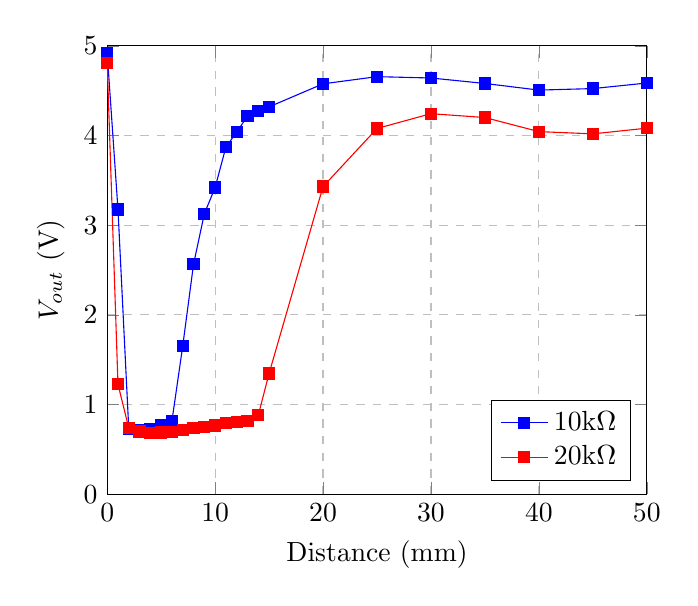
\begin{tikzpicture}
        \begin{axis} [
            xlabel={Distance (mm)},
            ylabel={$V_{out}$ (V)}, % might need to change this
            xmin=0, xmax=50,
            ymin=0, ymax=5,
            ymajorgrids=true,
            xmajorgrids=true,
            legend pos=south east,
            grid style=dashed,
        ]
            \addplot[
                color=blue,
                mark=square*
            ]
            coordinates {
                (0, 4.919)
                (1, 3.175)
                (2, 0.727)
                (3, 0.71)
                (4, 0.729)
                (5, 0.771)
                (6, 0.817)
                (7, 1.652)
                (8, 2.563)
                (9, 3.126)
                (10, 3.42)
                (11, 3.871)
                (12, 4.038)
                (13, 4.216)
                (14, 4.274)
                (15, 4.319)
                (20, 4.576)
                (25, 4.656)
                (30, 4.641)
                (35, 4.58)
                (40, 4.506)
                (45, 4.523)
                (50, 4.585)
            };
            \addlegendentry{10k$\Omega$}

            \addplot[
                color=red,
                mark=square*
            ]
            coordinates {
                (0, 4.81)
                (1, 1.225)
                (2, 0.7372)
                (3,0.6984)
                (4, 0.6831)
                (5, 0.6874)
                (6,0.6971)
                (7, 0.7156)
                (8, 0.735)
                (9, 0.7514)
                (10,0.765)
                (11, 0.7899)
                (12, 0.8059)
                (13, 0.82)
                (14, 0.8802)
                (15, 1.346)
                (20, 3.43)
                (25, 4.078)
                (30, 4.243)
                (35,4.2)
                (40, 4.043)
                (45, 4.018)
                (50, 4.0815)
            };
            \addlegendentry{20k$\Omega$}
        \end{axis}
    \end{tikzpicture}
    \caption{Distance of Reflective Surface from OPB745 vs Voltage}
    \label{distanceVoltageFigure}
\end{figure}

Fig.~\ref{distanceVoltageFigure} shows the voltage in both cases start at near the
logic high voltage and immediately drop, and then rise more
gradually back up to about 0.5 or 1.0 volts lower, for the
10k$\omega$ case and 20k$\omega$ case respectively. From these
voltage values, a current relationship could also be calculated
by subtracted $V_{out}$, that being the voltage across the
phototransistor, from the logic high voltage of 5 volts, which
gives the voltage across the resistor, and then using Ohm's law
to determine the current by dividing by the resistance. The
outcome of these calculations is shown in Fig.~\ref{distanceCurrentFigure}

\begin{figure}[htbp]
    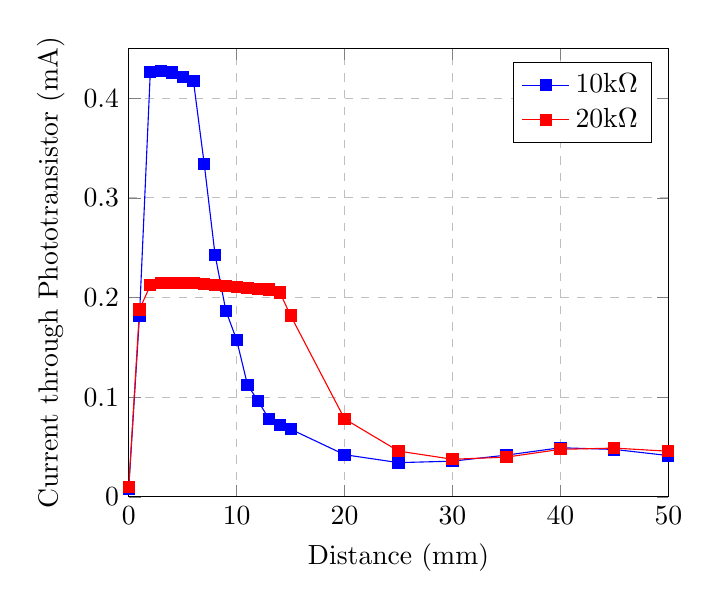
\begin{tikzpicture}
        \begin{axis} [
            xlabel={Distance (mm)},
            ylabel={Current through Phototransistor (mA)}, % might need to change this
            xmin=0, xmax=50,
            ymin=0, ymax=0.45,
            ymajorgrids=true,
            xmajorgrids=true,
            legend pos=north east,
            grid style=dashed,
        ]
            \addplot[
                color=blue,
                mark=square*
            ]
            coordinates {
                (0,  0.008077383)
                (1,  0.181990427)
                (2,  0.426106901)
                (3,  0.427802154)                
                (4,  0.425907459)
                (5,  0.421719186)
                (6,  0.41713203 )
                (7,  0.333865178)
                (8,  0.243019545)
                (9,  0.186876745)
                (10, 0.157558835)                
                (11, 0.112584763)
                (12, 0.095931392)
                (13, 0.078111288)
                (14, 0.072397288)
                (15, 0.067909852)
                (20, 0.042281611)
                (25, 0.034303949)
                (30, 0.035799761)
                (35, 0.041882728)                
                (40, 0.049262066)
                (45, 0.047566813)
                (50, 0.041384124)
            };
            \addlegendentry{10k$\Omega$}

            \addplot[
                color=red,
                mark=square*
            ]
            coordinates {
                (0,  0.009462151)      
                (1,  0.187998008)       
                (2,  0.212290837)        
                (3,  0.214223108)        
                (4,  0.21498506 )        
                (5,  0.214770916)        
                (6,  0.214287849)        
                (7,  0.213366534)        
                (8,  0.212400398)       
                (9,  0.211583665)        
                (10, 0.210906375)       
                (11, 0.209666335)        
                (12, 0.208869522)        
                (13, 0.208167331)      
                (14, 0.205169323)        
                (15, 0.181972112)       
                (20, 0.078187251)      
                (25, 0.045916335)       
                (30, 0.037699203)       
                (35, 0.039840637)     
                (40, 0.047659363)       
                (45, 0.048904382)       
                (50, 0.045742032)        
            };
            \addlegendentry{20k$\Omega$}
        \end{axis}
    \end{tikzpicture}
    \caption{Distance of Reflective Surface from OPB745 vs Current}
    \label{distanceCurrentFigure}
\end{figure}

Fig.~\ref{distanceVoltageFigure} and Fig.~\ref{distanceCurrentFigure}
show the relationship between the distance of the reflective
material and the voltage and current associated with the
phototransistor in the OPB745. This data demonstrates three
stages within the relationship. 

When the voltage across the phototransistor is high and
the current through it is low, this means that the phototransistor is
less active, and a low voltage and higher current means
the phototransistor is more active. Therefore, in the first
stage, where the voltage is very high and the current is very
low, it is clear that the phototransistor is receiving almost
no light from the infrared diode. This is due to the fact
that the reflective coating is so close that the light from
the diode cannot escape the OPB745, leading to very little entering
the phototransistor.

In the next stage, the reflective material is far enough
from the OPB745 to allow light to exit, and due to the close
proximity, much is reflected directly into the phototransistor.
This causes the low voltage and high current seen in the data
after the dropoff from the first stage.

When the reflective material is moved far enough from the
device to allow reflected light to scatter to areas
other than the phototransistor, the voltage quickly rises and
the current falls. The values settle at a level that is
less extreme than the initial near-complete occlusion of
the phototransistor, as some light still reaches it.

\subsection{Maintaining the Integrity of the Specifications}

The IEEEtran class file is used to format your paper and style the text. All margins, 
column widths, line spaces, and text fonts are prescribed; please do not 
alter them. You may note peculiarities. For example, the head margin
measures proportionately more than is customary. This measurement 
and others are deliberate, using specifications that anticipate your paper 
as one part of the entire proceedings, and not as an independent document. 
Please do not revise any of the current designations.

\section{Prepare Your Paper Before Styling}
Before you begin to format your paper, first write and save the content as a 
separate text file. Complete all content and organizational editing before 
formatting. Please note sections \ref{AA}--\ref{SCM} below for more information on 
proofreading, spelling and grammar.

Keep your text and graphic files separate until after the text has been 
formatted and styled. Do not number text heads---{\LaTeX} will do that 
for you.

\subsection{Abbreviations and Acronyms}\label{AA}
Define abbreviations and acronyms the first time they are used in the text, 
even after they have been defined in the abstract. Abbreviations such as 
IEEE, SI, MKS, CGS, ac, dc, and rms do not have to be defined. Do not use 
abbreviations in the title or heads unless they are unavoidable.

\subsection{Units}
\begin{itemize}
\item Use either SI (MKS) or CGS as primary units. (SI units are encouraged.) English units may be used as secondary units (in parentheses). An exception would be the use of English units as identifiers in trade, such as ``3.5-inch disk drive''.
\item Avoid combining SI and CGS units, such as current in amperes and magnetic field in oersteds. This often leads to confusion because equations do not balance dimensionally. If you must use mixed units, clearly state the units for each quantity that you use in an equation.
\item Do not mix complete spellings and abbreviations of units: ``Wb/m\textsuperscript{2}'' or ``webers per square meter'', not ``webers/m\textsuperscript{2}''. Spell out units when they appear in text: ``. . . a few henries'', not ``. . . a few H''.
\item Use a zero before decimal points: ``0.25'', not ``.25''. Use ``cm\textsuperscript{3}'', not ``cc''.)
\end{itemize}

\subsection{Equations}
Number equations consecutively. To make your 
equations more compact, you may use the solidus (~/~), the exp function, or 
appropriate exponents. Italicize Roman symbols for quantities and variables, 
but not Greek symbols. Use a long dash rather than a hyphen for a minus 
sign. Punctuate equations with commas or periods when they are part of a 
sentence, as in:
\begin{equation}
a+b=\gamma\label{eq}
\end{equation}

Be sure that the 
symbols in your equation have been defined before or immediately following 
the equation. Use ``\eqref{eq}'', not ``Eq.~\eqref{eq}'' or ``equation \eqref{eq}'', except at 
the beginning of a sentence: ``Equation \eqref{eq} is . . .''

\subsection{\LaTeX-Specific Advice}

Please use ``soft'' (e.g., \verb|\eqref{Eq}|) cross references instead
of ``hard'' references (e.g., \verb|(1)|). That will make it possible
to combine sections, add equations, or change the order of figures or
citations without having to go through the file line by line.

Please don't use the \verb|{eqnarray}| equation environment. Use
\verb|{align}| or \verb|{IEEEeqnarray}| instead. The \verb|{eqnarray}|
environment leaves unsightly spaces around relation symbols.

Please note that the \verb|{subequations}| environment in {\LaTeX}
will increment the main equation counter even when there are no
equation numbers displayed. If you forget that, you might write an
article in which the equation numbers skip from (17) to (20), causing
the copy editors to wonder if you've discovered a new method of
counting.

{\BibTeX} does not work by magic. It doesn't get the bibliographic
data from thin air but from .bib files. If you use {\BibTeX} to produce a
bibliography you must send the .bib files. 

{\LaTeX} can't read your mind. If you assign the same label to a
subsubsection and a table, you might find that Table I has been cross
referenced as Table IV-B3. 

{\LaTeX} does not have precognitive abilities. If you put a
\verb|\label| command before the command that updates the counter it's
supposed to be using, the label will pick up the last counter to be
cross referenced instead. In particular, a \verb|\label| command
should not go before the caption of a figure or a table.

Do not use \verb|\nonumber| inside the \verb|{array}| environment. It
will not stop equation numbers inside \verb|{array}| (there won't be
any anyway) and it might stop a wanted equation number in the
surrounding equation.

\subsection{Some Common Mistakes}\label{SCM}
\begin{itemize}
\item The word ``data'' is plural, not singular.
\item The subscript for the permeability of vacuum $\mu_{0}$, and other common scientific constants, is zero with subscript formatting, not a lowercase letter ``o''.
\item In American English, commas, semicolons, periods, question and exclamation marks are located within quotation marks only when a complete thought or name is cited, such as a title or full quotation. When quotation marks are used, instead of a bold or italic typeface, to highlight a word or phrase, punctuation should appear outside of the quotation marks. A parenthetical phrase or statement at the end of a sentence is punctuated outside of the closing parenthesis (like this). (A parenthetical sentence is punctuated within the parentheses.)
\item A graph within a graph is an ``inset'', not an ``insert''. The word alternatively is preferred to the word ``alternately'' (unless you really mean something that alternates).
\item Do not use the word ``essentially'' to mean ``approximately'' or ``effectively''.
\item In your paper title, if the words ``that uses'' can accurately replace the word ``using'', capitalize the ``u''; if not, keep using lower-cased.
\item Be aware of the different meanings of the homophones ``affect'' and ``effect'', ``complement'' and ``compliment'', ``discreet'' and ``discrete'', ``principal'' and ``principle''.
\item Do not confuse ``imply'' and ``infer''.
\item The prefix ``non'' is not a word; it should be joined to the word it modifies, usually without a hyphen.
\item There is no period after the ``et'' in the Latin abbreviation ``et al.''.
\item The abbreviation ``i.e.'' means ``that is'', and the abbreviation ``e.g.'' means ``for example''.
\end{itemize}
An excellent style manual for science writers is \cite{b7}.

\subsection{Authors and Affiliations}
\textbf{The class file is designed for, but not limited to, six authors.} A 
minimum of one author is required for all conference articles. Author names 
should be listed starting from left to right and then moving down to the 
next line. This is the author sequence that will be used in future citations 
and by indexing services. Names should not be listed in columns nor group by 
affiliation. Please keep your affiliations as succinct as possible (for 
example, do not differentiate among departments of the same organization).

\subsection{Identify the Headings}
Headings, or heads, are organizational devices that guide the reader through 
your paper. There are two types: component heads and text heads.

Component heads identify the different components of your paper and are not 
topically subordinate to each other. Examples include Acknowledgments and 
References and, for these, the correct style to use is ``Heading 5''. Use 
``figure caption'' for your Figure captions, and ``table head'' for your 
table title. Run-in heads, such as ``Abstract'', will require you to apply a 
style (in this case, italic) in addition to the style provided by the drop 
down menu to differentiate the head from the text.

Text heads organize the topics on a relational, hierarchical basis. For 
example, the paper title is the primary text head because all subsequent 
material relates and elaborates on this one topic. If there are two or more 
sub-topics, the next level head (uppercase Roman numerals) should be used 
and, conversely, if there are not at least two sub-topics, then no subheads 
should be introduced.

\subsection{Figures and Tables}
\paragraph{Positioning Figures and Tables} Place figures and tables at the top and 
bottom of columns. Avoid placing them in the middle of columns. Large 
figures and tables may span across both columns. Figure captions should be 
below the figures; table heads should appear above the tables. Insert 
figures and tables after they are cited in the text. Use the abbreviation 
``Fig.~\ref{fig}'', even at the beginning of a sentence.

\begin{table}[htbp]
\caption{Table Type Styles}
\begin{center}
\begin{tabular}{|c|c|c|c|}
\hline
\textbf{Table}&\multicolumn{3}{|c|}{\textbf{Table Column Head}} \\
\cline{2-4} 
\textbf{Head} & \textbf{\textit{Table column subhead}}& \textbf{\textit{Subhead}}& \textbf{\textit{Subhead}} \\
\hline
copy& More table copy$^{\mathrm{a}}$& &  \\
\hline
\multicolumn{4}{l}{$^{\mathrm{a}}$Sample of a Table footnote.}
\end{tabular}
\label{tab1}
\end{center}
\end{table}

\begin{figure}[htbp]
\centerline{
\includegraphics{fig1.png}}
\caption{Example of a figure caption.}
\label{fig}
\end{figure}

Figure Labels: Use 8 point Times New Roman for Figure labels. Use words 
rather than symbols or abbreviations when writing Figure axis labels to 
avoid confusing the reader. As an example, write the quantity 
``Magnetization'', or ``Magnetization, M'', not just ``M''. If including 
units in the label, present them within parentheses. Do not label axes only 
with units. In the example, write ``Magnetization (A/m)'' or ``Magnetization 
\{A[m(1)]\}'', not just ``A/m''. Do not label axes with a ratio of 
quantities and units. For example, write ``Temperature (K)'', not 
``Temperature/K''.

\section*{Acknowledgment}

The preferred spelling of the word ``acknowledgment'' in America is without 
an ``e'' after the ``g''. Avoid the stilted expression ``one of us (R. B. 
G.) thanks $\ldots$''. Instead, try ``R. B. G. thanks$\ldots$''. Put sponsor 
acknowledgments in the unnumbered footnote on the first page.

\section*{References}

Please number citations consecutively within brackets \cite{b1}. The 
sentence punctuation follows the bracket \cite{b2}. Refer simply to the reference 
number, as in \cite{b3}---do not use ``Ref. \cite{b3}'' or ``reference \cite{b3}'' except at 
the beginning of a sentence: ``Reference \cite{b3} was the first $\ldots$''

Number footnotes separately in superscripts. Place the actual footnote at 
the bottom of the column in which it was cited. Do not put footnotes in the 
abstract or reference list. Use letters for table footnotes.

Unless there are six authors or more give all authors' names; do not use 
``et al.''. Papers that have not been published, even if they have been 
submitted for publication, should be cited as ``unpublished'' \cite{b4}. Papers 
that have been accepted for publication should be cited as ``in press'' \cite{b5}. 
Capitalize only the first word in a paper title, except for proper nouns and 
element symbols.

For papers published in translation journals, please give the English 
citation first, followed by the original foreign-language citation \cite{b6}.

\begin{thebibliography}{00}
\bibitem{b1} G. Eason, B. Noble, and I. N. Sneddon, ``On certain integrals of Lipschitz-Hankel type involving products of Bessel functions,'' Phil. Trans. Roy. Soc. London, vol. A247, pp. 529--551, April 1955.
\bibitem{b2} J. Clerk Maxwell, A Treatise on Electricity and Magnetism, 3rd ed., vol. 2. Oxford: Clarendon, 1892, pp.68--73.
\bibitem{b3} I. S. Jacobs and C. P. Bean, ``Fine particles, thin films and exchange anisotropy,'' in Magnetism, vol. III, G. T. Rado and H. Suhl, Eds. New York: Academic, 1963, pp. 271--350.
\bibitem{b4} K. Elissa, ``Title of paper if known,'' unpublished.
\bibitem{b5} R. Nicole, ``Title of paper with only first word capitalized,'' J. Name Stand. Abbrev., in press.
\bibitem{b6} Y. Yorozu, M. Hirano, K. Oka, and Y. Tagawa, ``Electron spectroscopy studies on magneto-optical media and plastic substrate interface,'' IEEE Transl. J. Magn. Japan, vol. 2, pp. 740--741, August 1987 [Digests 9th Annual Conf. Magnetics Japan, p. 301, 1982].
\bibitem{b7} M. Young, The Technical Writer's Handbook. Mill Valley, CA: University Science, 1989.
\end{thebibliography}

\end{document}
